\chapter{Implementation}\label{Chap:Implementation}

In this chapter I will write about some implementation aspects that were interesting or problematic during the development of the PARRHI system. For that, I will use a bottom down strategy, meaning, that I will talk about the general setup of the implemented system, and then drill down into the components. I will explain what software was used, why I made these decisions and whether or not they where good or bad in hindsight.

\section{PARRHI Hardware}
For the Augmented Reality purposes, I decided to use the first version of Microsoft's Augmented Reality glass called HoloLens~\cite{HoloLens}. The HoloLans has all needed capabilities like cameras for image and environment tracking, simple hand gesture recognition, a reasonably good field of view and was programmable with the 3D game engine Unity. The TUM chair of "Automation and Information Systems (AIS)" thankfully supplied me with this product.

The second main hardware component in the PARRHI system is the Robot. The robot manufacturing company Fanuc~\cite{Fanuc} was gracious enough to gift the TUM chair "Automation and Information Systems (AIS)" a free CR-7iA/L collaborative, 6 DOF, industrial robot~\cite{FanucCR7} and a R-30iB controller~\cite{FanucR30iB}. The R-30iB controller than can either be programmed in Fanuc's TP-Language or in Fanuc's KAREL language. KAREL offers many possibilities with network sockets, reading and writing data from and to the robot's controller, whereas TP programmes are fit for moving and steering the robot.

The last component is a gripper provided by SCHUNK. The company gifted us a collaborative Co-act EGP-C~\cite{SchunkGripper}, that seamlessly integrated into the Fanuc robot with a hardware interface for exactly that purpose. 

At this point I would like to thank both Fanuc and Schunk massively for their supplies, so that this bachelor's thesis could be realised.

%4) Implementation
%- Introduction into the implementation, Main language
%4.1) PARRHI System and setup
\section{PARRHI Software}
%- Generally: Some things in library, some things in Unity
Software Implementation wise, the PARRHI system is split up in three big components. First there is the PARRHI library, secondly the Robot library and lastly the Unity engine. The PARRHI library is the most intelligent component, since it contains all the logic for the Real World Model, the Parametrised Program, the Core Routine and commands the Input and Output Modules (see fig.~\ref{Fig:PARRHIConcept}). The Robot library has the tools necessary to communicate with the Robot in the Real World and is used by the Input and Output Modules. The third component \textit{Unity} hosts the PARRHI runtime library, and handles the AR-World, network communication etc.


\begin{figure}[!h]
	\centering
	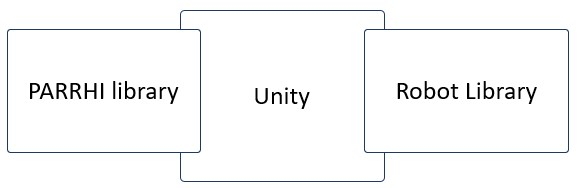
\includegraphics[width=0.5\textwidth]{Figures/Implementation_SystemSetup.jpg}
	\caption{PARRHI implementation setup}
	\label{Fig:Implementation}
\end{figure}


%4.2) PARRHI Library
\section{PARRHI Library}
%- Build up, workflow, interesting things
The PARRHI system was programmed in Microsoft's .NET framework version 4.6.1~\cite{NETFramework} using $C\#$ \cite{CSharp}. Besides being my personal preference, this decision was made because the Unity game engine is used with the language $C\#$. The PARRHI library itself is a \textit{Class Library} project~\cite{ClassLibrary} and has three main tasks.

\begin{enumerate}
	\item Import the Parametrised Program and perform some operations on it. The Parametrised Program is a XML~\cite{xmlW3C} based document. After importing it is validated using an XSD~\cite{xsdW3C} document. Finally the PARRHI library has to extract useable $C\#$ objects from the deserialized XML document and setup references.
	\item It contains the Real World Model and the logic behind it. In my specific case, this means, that the PARRHI library contains the Robot's forward kinematics model and the required information to convert the HoloLens' internal coordinates, into the robot's coordinate system.
	\item The Core Routine is located in the PARRHI library, meaning, that on every iteration the PARRHI system calls into the PARRHI library to perform its task.
\end{enumerate}

Importing and validating the XML document is very easy, since the used .NET framework natively supports that. The implementation of the PARRHI Core Routine is also quite straight forward, which is why I will not talk about it too much. More interesting is the Robot's forwards kinematics, which will be presented now.

\subsection{CR-i7A Forward Kinematics}
In robotics a robot can be described in two different spaces. On one hand there is the joint space meaning, that all vectors represent joints and are related to their angles. Since the robot has six joints, the joint space is six dimensional. In the joint space the position vector is often represented as $ \vec{q} $.

On the other hand there is the task-space. In this space, the position vector represents the robot's tip in Cartesian coordinates. If the joint space is six dimension, then generally speaking the task space is also six dimensional and represented as follows, with $x,y,z$ being the 3D coordinates, and $\alpha, \beta, \gamma $ being the orientation of the tip.
\[ \vec{q} = \begin{pmatrix} q_1 \\ q_2 \\ q_3 \\ q_4 \\ q_5 \\ q_6 \end{pmatrix}, \vec{x} = \begin{pmatrix} x \\ y \\ z \\ \alpha \\ \beta \\ \gamma \\ \end{pmatrix} with~~\vec{x},\vec{q} \in \mathbb{R}^6  \]. 

The forward kinematics now describes the process of transitioning form $ \vec{q} $ to $ \vec{x} $. This is done as follows: $ \vec{x} = f(\vec{q})~~~( \mathbb{R}^6 \rightarrow \mathbb{R}^6)$. Where the mapping $f$ depends on the robot's specific configuration and geometric properties.

To calculate $f$, I first defined local Cartesian coordinate systems after each joint. In fig.~\ref{Fig:ForwardKinematics} the green axes represent the robot, and the black vectors represent the coordinate systems $\phi_i = (x_i, y_i, z_i)$, and $l_i$ represent the axes defined in the coordinate system $\phi_i$.

\begin{figure}[h!]
	\begin{minipage}{0.45\textwidth}
		\centering
		
\tdplotsetmaincoords{60}{120} 
\begin{tikzpicture}  [scale=0.08, tdplot_main_coords, axis/.style={->, black, thin}, 
vector/.style={-stealth,green,very thick}, 
robot/.style={green, very thick},
vector guide/.style={dashed,gray,thin}]

\usetikzlibrary{calc}

%standard tikz coordinate definition using x, y, z coords
\coordinate (O) at (0,0,0);

%tikz-3dplot coordinate definition using x, y, z coords


\pgfmathsetmacro{\axSize}{100}
\pgfmathsetmacro{\saxSize}{10}
\pgfmathsetmacro{\jointRadius}{30}

%Robot Points in cm (mm too large dimensions for library)
\coordinate (P0) at (0,0,0);
\coordinate (P1) at (5,0,33);
\coordinate (P2) at (5, 0, 77);
\coordinate (P25) at (10, 0, 100.5);
\coordinate (P3) at (15, 0, 100.5);
\coordinate (P4) at (47, 0, 100.5);
\coordinate (P5) at (55, 0, 100.5);
\coordinate (P6) at (63, 0, 100.5);


%draw coordinate system axes
%\draw[axis] (0,0,0) -- (\axSize,0,0) node[anchor=north east]{$x$};
%\draw[axis] (0,0,0) -- (0,\axSize,0) node[anchor=north west]{$y$};
%\draw[axis] (0,0,0) -- (0,0,\axSize) node[anchor=south]{$z$};


\draw[axis] (P0) -- (\saxSize,0,0) node[anchor=north east]{$x_0$};
\draw[axis] (P0) -- (0,\saxSize,0) node[anchor=north west]{$y_0$};
\draw[axis] (P0) -- (0,0,\saxSize) node[anchor=west]{$z_0$};

\draw[axis] (P1) -- ($ (P1) + (\saxSize,0,0)$) node[anchor=north east]{$x_1$};
\draw[axis] (P1) -- ($ (P1) + (0,\saxSize,0)$) node[anchor=north west]{$y_1$};
\draw[axis] (P1) -- ($ (P1) + (0,0,\saxSize)$) node[anchor=west]{$z_1$};

\draw[axis] (P2) -- ($ (P2) + (\saxSize,0,0)$) node[anchor=north east]{$x_2$};
\draw[axis] (P2) -- ($ (P2) + (0,\saxSize,0)$) node[anchor=north]{$y_2$};
\draw[axis] (P2) -- ($ (P2) + (0,0,\saxSize)$) node[anchor=south]{$z_2$};

\draw[axis] (P3) -- ($ (P3) + (\saxSize,0,0)$) node[anchor=south east]{$x_3$};
\draw[axis] (P3) -- ($ (P3) + (0,\saxSize,0)$) node[anchor=north west]{$y_3$};
\draw[axis] (P3) -- ($ (P3) + (0,0,\saxSize)$) node[anchor=south]{$z_3$};

\draw[axis] (P4) -- ($ (P4) + (\saxSize,0,0)$) node[anchor=south east]{$x_4$};
\draw[axis] (P4) -- ($ (P4) + (0,\saxSize,0)$) node[anchor=south west]{$y_4$};
\draw[axis] (P4) -- ($ (P4) + (0,0,\saxSize)$) node[anchor=south]{$z_4$};

\draw[axis] (P5) -- ($ (P5) + (\saxSize,0,0)$) node[anchor=north east]{$x_5$};
\draw[axis] (P5) -- ($ (P5) + (0,\saxSize,0)$) node[anchor=north east]{$y_5$};
\draw[axis] (P5) -- ($ (P5) + (0,0,\saxSize)$) node[anchor=south]{$z_5$};

%draw the robot's joints and axes
\draw[robot] (P0) -- (P1); \fill[fill=gray] (P0) circle (\jointRadius pt);
\draw[robot] (P1) -- (P2); \fill[fill=gray] (P1) circle (\jointRadius pt);
\draw[robot] (P2) -- (P25); \fill[fill=gray] (P2) circle (\jointRadius pt);
\draw[robot] (P25) -- (P3); 
\draw[robot] (P3) -- (P4); \fill[fill=gray] (P3) circle (\jointRadius pt);
\draw[robot] (P4) -- (P5); \fill[fill=gray] (P4) circle (\jointRadius pt);
\draw[robot] (P5) -- (P6); \fill[fill=gray] (P5) circle (\jointRadius pt);

%draw the 
\node[tdplot_main_coords,anchor=east] at ($(P0) + (10,0,15)$){$\vec{l_0}$};
\node[tdplot_main_coords,anchor=east] at ($(P1) + (5,0,20)$){$\vec{l_1}$};
\node[tdplot_main_coords,anchor=east] at ($(P2) + (-12,0,00)$){$\vec{l_2}$};
\node[tdplot_main_coords,anchor=east] at ($(P3) + (10,0,10)$){$\vec{l_3}$};
\node[tdplot_main_coords,anchor=south east] at ($(P4) + (-1,1,0)$){$\vec{l_4}$};
\node[tdplot_main_coords,anchor=north] at ($(P5) + (0,0,0)$){$\vec{l_5}$};




\end{tikzpicture}
		\caption{Robot-Point example}
		\label{Fig:ForwardKinematics}
	\end{minipage}\hfill
	\begin{minipage}{0.45\textwidth}
		The following matrices ($\phi_i$) allow the conversion from vectors expressed in the coordinate system $n + 1$ to the expression in system $n$, with $\vec{l_n} = \phi_{n+1}(q_{n+1}) * \vec{l_{n+1}}$. After transforming the vector $\vec{l_{n+1}}$ into the coordinate system $\phi_n$ one can add the vector $\vec{l_n}$
	\end{minipage}
\end{figure}
	
%4.3) Unity structure
\section{Unity}
%- What is unity?




%4.3.1) General Setup
\subsection{General Unity Setup}
%- How is library implemented



%4.3.2) Image Tracking
\subsection{Image Tracking}
%- Vuforia Engine



%4.3.3) ARToolkit%
\subsection{AR-Toolkit}
%- AR Toolkit explanation and usage



%4.4) Robot Protocol
\section{Robot Library}
%- Strucutre, languages, problems, solutions



%4.5) Parametrised Program Validation and Definition
\section{Parametrised Program Implementation and Validation}
%- XML leads to C# classes etc.



%4.4.1) XML Structure
\subsection{XML Structure}
%%- Give XML Tags



%4.4.2) XSD generation and validation#
\subsection{XSD generation and validation}
%- Auto generate xsd and c# classes